\documentclass[main.tex]{subfiles}
\begin{document}


\section{Фермионы}\label{ch15}

\subsection{Преобразование Джордана-Вигнера}\label{ch15.1}

Чтобы найти более точные связи между реальным квантовым миром, с одной стороны, и детерминированными моделями автоматов, с другой, требуется гораздо больше математических механизмов. Для начала, можно в элегантной манере обработать фермионы.

Возьмем детерминированную модель с $М$ состояниями. Пример, описанный на рис. \ref{i2.2}, представляет собой модель с $M = 31$ состоянием, а закон эволюции для одного временного шага представляет собой элемент P группы перестановок для $M = 31$ элемента: $P\in P_M$. Пусть его состояния обозначены как $|1\rangle,\ldots,|M\rangle$. Мы записываем один шаг эволюции как:

\begin{equation}\label{15.1}
	|i\rangle_{t} \rightarrow|i\rangle_{t+\delta t}=|P(i)\rangle_{t}=\sum_{j=1}^{M} P_{i j}|j\rangle_{t}, \quad i=1, \ldots, M
\end{equation}

где последняя матрица $P$ имеет матричные элементы $\langle j|P|i \rangle$, которые состоят из 0 и 1, при этом, в каждой строке и в каждом столбце по одной единице. Как объяснено в разделе \ref{ch2.2.2}, мы предполагаем, что матрица Гамильтона $\hat H_{ij}$ определена так, что (при нормализации шага времени $\delta t$ к единице)

\begin{equation}\label{15.2}
	\langle j|P| i\rangle=\left(e^{-i H^{\mathrm{op}}}\right)_{j i}
\end{equation}
         
где, возможно, может быть добавлена энергия $\delta E$ нулевой точки, которая есть сохраняющаяся величина: $\delta E$ зависит только от цикла, к которому принадлежит индекс $i$, но не от элемента внутри цикла.

Теперь мы свяжем с этой моделью другую, чьи переменные являются булевыми, принимая значения 0 или 1 (или, что эквивалентно, $+ 1$ или $-1$) в каждом из этих $M$ состояний. Это означает, что в нашем примере мы имеем $2^M = 2, 147, 483, 648$ состояний, одно из которых показано на рис. \ref{i15.1}. Закон эволюции определен так, что эти булевы числа перемещаются так же, как состояния в исходной модели зубчатого колеса. Физически это означает, что, если в исходной модели ровно одна частица двигалась по заданному правилу, то теперь у нас есть $N$ движущихся частиц, где $N$ может варьироваться от 0 до $М$. В физике элементарных частиц это известно как «вторичное квантование». Поскольку две частицы не могут находиться на одном месте, выходит, что у нас есть фермионы, подчиняющиеся принципу исключения Паули.


\begin{figure}[ht]
\begin{center}
\scalebox{0.4}{
   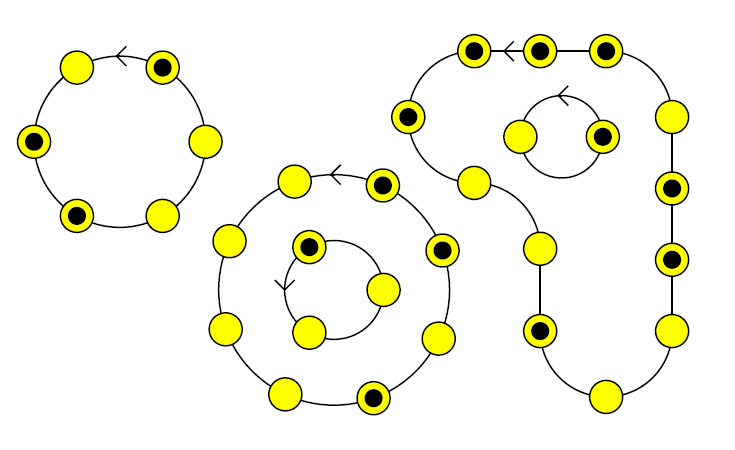
\includegraphics{images/img_15_1.png}
}
\caption{
\label{i15.1} <<Вторично-квантованная>> версия модели с несколькими зубчатыми колесами на фиг. 2.2. Черные точки представляют собой фермионы}
\end {center}
\end {figure}

Чтобы описать эти детерминированные фермионы в квантово-механической записи, сначала введем операторные поля $\hat\phi_i$, выступающие в качестве операторов аннигиляции, и их эрмитовы сопряженные $\hat\phi_i^\dagger$, которые действуют как операторы рождения. Обозначая наши состояния как $| n_1, n_2,\ldots,n_M\rangle$, где все $n$ равны 0 или 1, мы постулируем

\begin{equation}\label{15.3}
	\begin{aligned} \phi_{i}^{\mathrm{op}}\left|n_{1}, \ldots, n_{i}, \ldots, n_{M}\right\rangle &= n_{i}\left|n_{1}, \ldots, n_{i}-1, \ldots, n_{M}\right\rangle \\ \phi_{i}^{\mathrm{op\dagger}}\left|n_{1}, \ldots, n_{i}, \ldots, n_{M}\right\rangle &=\left(1-n_{i}\right)\left|n_{1}, \ldots, n_{i}+1, \ldots, n_{M}\right\rangle \end{aligned}
\end{equation}

В конкретном состоянии $i$ эти поля подчиняются правилам (для краткости опущен верхний индекс 'op'):

\begin{equation}\label{15.4}
	\left(\phi_{i}\right)^{2}=0, \quad \phi_{i}^{\dagger} \phi_{i} + \phi_{i} \phi_{i}^{\dagger} = \mathbb{I}
\end{equation}

где $\mathbb{I}$ - тождественный оператор; на разных состояниях поля коммутируют: $\phi_i\phi_j = \phi_j\phi_i$, $\phi_i^\dagger\phi_j = \phi_j\phi_i^\dagger$, $i \neq j$.
Чтобы превратить их в полностью антикоммутирующие (фермионные) поля, мы применяем так называемое преобразование Джордана-Вигнера [54]:

\begin{equation}\label{15.5}
	\psi_{i}=(-1)^{n_{1}+\cdots+n_{i-1}} \phi_{i}
\end{equation}
          
где $n_i = \phi_i \phi_i^\dagger = \psi_i \psi_i^\dagger$ - номера заполнения на $i$-ом состоянии , т.е. мы вставляем знак минус, если занято нечетное количество состояний $j<i$. В результате этой хорошо известной процедуры

\begin{equation}\label{15.6}
	\psi_{i} \psi_{j}+\psi_{j} \psi_{i}=0, \quad \psi_{i}^{\dagger} \psi_{j}+\psi_{j} \psi_{i}^{\dagger}=\delta_{i j}, \quad \forall(i, j)
\end{equation}

Достоинство этого преобразования заключается в том, что антикоммутационные соотношения (\ref{15.6}) остаются неизменными после любого линейного унитарного преобразования $\psi_i$, как векторов в нашем М-мерном векторном пространстве, при условии, что $\psi_i^\dagger$ преобразуется как контравекторы. Обычно, минус в уравнении (\ref{15.5}) не вредит, но требуется некоторая осторожность.

Теперь рассмотрим матрицу перестановок $P$ и запишем гамильтониан в формуле (\ref{15.2}) в нижнем регистре $h_{ij}$; это матрица компонентов $M \times M$. Записав $U_{ij}(t) = (e^{-iht})_{ij}$, на целочисленных временных шагах получаем $\hat P_t = \hat U(t)$. Теперь мы утверждаем, что перестановка, которая перемещает фермионы, генерируется гамильтонианом $\hat H$

\begin{equation}\label{15.7}
	\hat H_{F} = \sum_{i j} \psi_{j}^{\dagger} h_{j i} \psi_{i}
\end{equation}

что доказывается следующим образом:             

\begin{equation}\label{15.8}
	\begin{aligned} \psi_{i}(t) &=e^{i H_{F}^{\mathrm{op}}} \psi_{i} e^{-i H_{F}^{\mathrm{op}} t} \\ \frac{\mathrm{d}}{\mathrm{d} t} e^{-i H_{F}^{\mathrm{op}} t} &=-i H_{F}^{\mathrm{op}} e^{-i H_{F}^{\mathrm{op}} t}=-i e^{-i H_{F}^{\mathrm{op}} t} H_{F}^{\mathrm{op}} \end{aligned}
\end{equation}
                                         
Тогда 

\begin{equation}\label{15.9}
	\begin{aligned} \frac{\mathrm{d}}{\mathrm{d} t} \psi_{k}(t) &=i e^{i H_{F}^{\mathrm{op}}} \sum_{i j}\left[\psi_{j}^{\dagger} h_{j i} \psi_{i}, \psi_{k}\right] e^{-i H_{F}^{\mathrm{op}} t} \\ &=i e^{i H_{F}^{\mathrm{op}} t} \sum_{i j} h_{j i}\left(-\left\{\psi_{j}^{\dagger}, \psi_{k}\right\} \psi_{i}+\psi_{j}^{\dagger}\left\{\psi_{i}, \psi_{k}\right\}\right) e^{-i H_{F}^{\mathrm{op}} t} \\ &=-i e^{i H_{F}^{\mathrm{op}} t} \sum_{i} h_{k i} \psi_{i} e^{-i H_{F}^{\mathrm{op}}t}=-i \sum_{i} h_{k i} \psi_{i}(t) \end{aligned}
\end{equation}

где $\{A, B\} = AB + BA$ - антикоммутатор (обратите внимание, что второй член во второй строке в уравнении (\ref{15.9}) обращается в нуль).

Это то же самое уравнение, которое описывает эволюцию состояний $| k\rangle$ исходной модели зубчатого колеса. Итак, мы видим, что на целых временных шагах $t$, поля $\psi_i(t)$ переставляются в соответствии с оператором перестановки $P_t$. Заметим теперь, что пустое состояние $| 0\rangle$ (которое не является вакуумным состоянием) вообще не эволюционирует (как и полностью заполненное состояние). Поэтому состояние N частиц ($0 \le N \le M$), полученное путем применения $N$ копий операторов поля $\psi_i^\dagger$, развивается с одним и тем же перестановочным устройством. Знак минус в формуле Джордана Вигнера (\ref{15.5}) дает преобразованному состоянию знак минус, если после $t$ перестановок порядок $N$ частиц стал нечетной перестановкой их первоначальных относительных положений. Хотя мы должны помнить о существовании этого минуса, в большинстве случаев он не играет существенной роли. Физически этот признак не наблюдается.

Важность показанной здесь процедуры заключается в том, что мы можем понять, как антикоммутирующие операторы фермионного поля $\psi_i$, или $\psi_i(x)$ могут возникнуть из детерминированного системы. Знаки минус в их (анти) коммутаторах обусловлены преобразованием Джордана-Вигнера (\ref{15.5}), без которого у нас не было бы вообще никаких коммутаторных выражений, так что вывод (\ref{15.11}) не удался бы.

Последний шаг в этой процедуре вторичного квантования состоит в том, что можно выполнить ортогональные преобразования между полями $\psi$ и $\psi^\dagger$, так чтобы расширить их в терминах собственных состояний $\psi_i(E_i)$ гамильтониана из одной частицы $h_{ij}$. Тогда состояние $| \emptyset \rangle$ подчиняется

\begin{equation}\label{15.12}
	\psi\left(E_{i}\right)|\emptyset\rangle= 0 \quad \text { if } E_{i}>0 ; \quad \psi^{\dagger}\left(E_{i}\right)|\emptyset\rangle= 0 \quad \text { if } \quad E_{i}<0
\end{equation}

и имеет самую низкую энергию. Это состояние вакуума, как предложил Дирак. Состояния с отрицательной энергией интерпретируются как дырки для античастиц. Операторы $\psi(E)$ аннигилируют частицы, если $E> 0$, или создают античастицы, если $E <0$. Для $\psi^\dagger(E)$ все наоборот. Частицы и античастицы теперь все несут положительную энергию. Является ли это решением проблемы, указанной в гл. \ref{ch14}? Это зависит от того, как мы обрабатываем взаимодействия, см. Гл. \ref{ch9.2}, и мы обсудим этот важный вопрос далее в разд. \ref{ch22.1} и в гл. \ref{ch23}.

Вывод этого раздела состоит в том, что, если гамильтонова матрица $h_{ij}$ описывает единственную или составную модель зубчатого колеса, приводящую к классическим перестановкам состояний $| i\rangle, i = 1,\ldots, M$, в целочисленные моменты времени, то модель с Гамильтонианом (\ref{15.7}) связана с системой, в которой занятые состояния эволюционируют в соответствии с одними и теми же перестановками, с той лишь разницей, что теперь общее число состояний составляет $2^M$ вместо $M$. И энергия всегда ограничена снизу.

Один объект, который в наибольшей степени является физической системой Гамильтона, не будет приводить к классическим перестановкам с целыми временными шагами, но наша модель - это только первый шаг. Следующим шагом может быть то, что $h_{ij}$ зависит от значений некоторых полей локальных операторов $\phi(x)$. Это то, что мы имеем в физическом мире, и это может произойти, если предположить, что правила перестановки для эволюции этих фермионных частиц зависят от других переменных в системе.

На самом деле, существует довольно реалистичная, упрощенная фермионная модель, в которой $h_{ij}$ действительно производит чистые перестановки. Это будет показано в следующем разделе.

Процедура для бозонов должна идти аналогичным образом, если речь идет о бозонных полях в квантовой теории поля. Однако связь с детерминированными теориями не так проста, как в фермионном случае, потому что в одном состоянии может находиться сколь угодно большое количество бозонных частиц. Чтобы смягчить эту ситуацию, было введено понятие гармонических ротаторов, которое также запрещает конечное число состояний. Мы можем применить более традиционное бозонное вторичное квантование в некоторых специальных двумерных теориях, см. Разд. \ref{ch17.1.1}.

Как вторичное квантование применяется в стандартных квантовых теориях поля, описано в разд. \ref{ch20.3}.


\subsection{«Нейтрино» в трех измерениях}\label{ch15.2}

В некоторых случаях начинают плясать от печки. Рассматривая типичную квантовую систему, можно ли разработать детерминированный классический автомат, который бы генерировал все его квантовые состояния? Сейчас покажем, как такой номер провернуть.

Один из способов определения, может ли квантовая система быть математически эквивалентной детерминированной модели, - это поиск полного набора beables. Как определено в разд. \ref{ch2.1.1}, beables - это операторы, которые могут описывать классические наблюдаемые, и поэтому они должны коммутировать друг друга всегда, всегда. Таким образом, для обычных квантовых частиц, таких как электрон, в водородной модели Бора, ни операторы $x$, ни $p$ не являются beables, потому что $[x (t), x (t ')] \neq 0$ и $[p (t), p (t') ] \neq 0$, при $t \neq t '$. Типичные модели, в которых мы имеем такие возможности, - это модели, в которых гамильтониан является линейным по импульсам, такие как в разд. \ref{ch12.3}, уравнение (\ref{12.17}), а не квадратичным по $p$. Ну а есть ли еще?

Возможно, beables образуют только сетку пространства-времени, тогда как данные о точках между точками на сетке не коммутируют. Это на самом деле хорошо послужило бы нашей цели, поскольку вполне возможно, что физические данные, характеризующие нашу вселенную, действительно формируют такую сетку, в то время как мы просто не можем наблюдать это, просто потому что сетка слишком хороша для современных инструментов и интерполяций, а выделение точек между ячейками сетки могло быть просто следствием нашего невежества.
Beables образуют полный набор, если в базисе, где все они диагональны, совокупность собственных значений полностью идентифицирует элементы этого базиса.

Насколько мы знаем сегодня, в Природе нет таких систем beables; то есть, если мы примем во внимание все известные силы, то все операторы, которые мы можем построить сегодня, прекратят коммутировать в некоторой точке. Мы можем и должны пытаться искать лучше, но, в качестве альтернативы, мы можем создавать упрощенные модели, описывающие только части того, что мы видим, которые позволяют преобразовывать в базис beables. В гл. \ref{12.1}, мы уже обсуждали гармонический ротатор в качестве важного примера, который пригодился для интересной математики в гл. \ref{13}. В конце концов, его большой предел $N$ должен воспроизводить обычный гармонический осциллятор. Здесь мы обсуждаем еще одну такую модель: безмассовые «нейтрино», в 3 пространственно-подобном и одном временоподобном измерении.

Один квантованный не взаимодействующий дираковский фермион подчиняется гамильтониану\footnote{Соглашение о суммировании: повторяющиеся индексы обычно суммируются.}

\begin{equation}\label{15.13}
	\hat H = \alpha_i p_i + \beta m
\end{equation}

где $\alpha_i$, $\beta$ - матрицы Дирака $4\times 4$, подчиняющиеся

\begin{equation}\label{15.14}
	\alpha_{i} \alpha_{j}+\alpha_{j} \alpha_{i}=2 \delta_{i j} ; \quad \beta^{2}=1 ; \quad \alpha_{i} \beta+\beta \alpha_{i}=0
\end{equation}

Только в случае $m = 0$ мы можем напрямую построить полный набор beables.\footnote{Массивные <<нейтрино>> можно рассматривать как безмассовые в пространстве с одним или несколькими дополнительными измерениями, и это тоже имеет под собой реальную основу. Однако проецирование этого набора обратно в 4 пространственно-временных измерения приводит к довольно надуманной конструкции.} В этом случае мы можем опустить матрицу $\beta$ и заменить $\sigma_i$ на три матрицы Паули, матрицы $2 \times 2$. Затем частицу можно рассматривать как безмассовое (майорановское или киральное) «нейтрино», имеющее только две компоненты в своей спинорной волновой функции. Нейтрино является полностью «стерильным», поскольку мы игнорируем любое из его взаимодействий. Вот почему мы называем это «нейтрино» с кавычками.

Здесь на самом деле есть два варианта: относительные знаки матриц Паули можно выбрать так, чтобы частицы имели положительную (левостороннюю) спиральность, а античастицы были правосторонними, или наоборот. Мы выбираем, что частицы имеют правосторонние спирали, если наша система координат $(x, y, z)$ ориентирована как пальцы 1,2,3 правой руки. Матрицы Паули подчиняются

\begin{equation}\label{15.15}
	\sigma_{1} \sigma_{2}=i \sigma_{3}, \quad \sigma_{2} \sigma_{3}=i \sigma_{1}, \quad \sigma_{3} \sigma_{1}=i \sigma_{2} ; \quad \sigma_{1}^{2}=\sigma_{2}^{2}=\sigma_{3}^{2}=1
\end{equation}

Beables тогда:

\begin{equation}\label{15.16}
	\begin{aligned}\left\{\mathcal{O}_{i}^{\mathrm{op}}\right\} &=\{\hat{q}, s, r\}, \quad \text { where } \\ \hat{q}_{i} \equiv \pm p_{i}/| p |, & s \equiv \hat{q} \cdot \vec{\sigma}, \quad r \equiv \frac{1}{2}(\hat{q} \cdot \vec{x}+\vec{x} \cdot \hat{q}) \end{aligned}
\end{equation}

Если быть точным, $\mathbf{q}$ - это единичный вектор, определяющий направление импульса по модулю его знака. Это означает, что мы записываем импульс $\vec p$ как

\begin{equation}\label{15.17}
	\vec p = p_r \hat q
\end{equation}

где $p_r$ может быть положительным или отрицательным вещественным числом. Это важно, потому что нам нужно его каноническое коммутационное отношение с переменной $r$, являющееся $[r, p_r] = i$, без дальнейших ограничений на $r$ или $p_r$. Если $p_r$ будет ограничено положительными числами $|p|$, то это подразумевает ограничения аналитичности для волновых функций $\psi(r)$.

Знак оператора $\hat{}$ напоминает нам, что это вектор единичной длины, $|\hat q| = 1$. Чтобы определить его знак, можно использовать условие $\hat q_z >0$. В качестве альтернативы, мы можем решить оставить симметрию $P_{int}$ (для «внутренней четности»),

\begin{equation}\label{15.18}
	\hat{q} \leftrightarrow-\hat{q}, \quad p_{r} \leftrightarrow-p_{r}, \quad r \leftrightarrow-r, \quad s \leftrightarrow-s
\end{equation}

после чего мы оставим только те волновые функции, которые четны после этого преобразования. Переменная $s$ может принимать только значения $s = \pm 1$, что можно проверить, взяв квадрат $\hat q \cdot \vec\sigma$. В дальнейшем символ будет зарезервирован для $\hat p = +\vec p/|p|$, так что $\hat q = \pm\hat p$.

Последний оператор в формуле (\ref{15.16}), оператор $r$, был симметризован, чтобы гарантировать, что он эрмитов. Это можно упростить, используя следующие наблюдения. В базисе $\vec p$ мы имеем

\begin{equation}\label{15.19}
	\begin{aligned} \vec{x}=i \frac{\partial}{\partial \vec{p}} ; \quad & \frac{\partial}{\partial \vec{p}} p_{r}=\hat{q} \\\left[x_{i}, p_{r}\right]=i \hat{q}_{i} ; &\left[x_{i}, \hat{q}_{j}\right]=\frac{i}{p_{r}}\left(\delta_{i j}-\hat{q}_{i} \hat{q}_{j}\right) \end{aligned}
\end{equation}

\begin{equation}\label{15.20}
	x_{i} \hat{q}_{i}-\hat{q}_{i} x_{i}=\frac{2 i}{p_{r}} \quad \rightarrow \quad \frac{1}{2}(\hat{q} \cdot \vec{x}+\vec{x} \cdot \hat{q})=\hat{q} \cdot \vec{x}+\frac{i}{p_{r}}
\end{equation}

Это можно проверить, разобрав случай $p_r = |p|>0$, $\hat q = \hat p$ и отметив, что все уравнения сохраняются при симметрии отражения (\ref{15.18}).

Легко проверить, что операторы (\ref{15.16}) действительно образуют полностью коммутирующий набор. Единственный нетривиальный коммутатор, который следует внимательно рассмотреть, - это $[r, \hat q] = [\hat q\cdot\vec x, \hat q]$.

Рассмотрим снова базис $\vec p$, где $\vec x = i\partial/\partial\vec p$: оператор $\vec p\cdot\partial/\partial\vec p$ является оператором растяжения. Но, поскольку $\hat q$ масштабно инвариантен, он коммутирует с этим оператором:

\begin{equation}\label{15.21}
	\left[\vec{p} \cdot \frac{\partial}{\partial \vec{p}}, \hat{q}\right]=0
\end{equation}

Следовательно

\begin{equation}\label{15.22}
	[\hat{q} \cdot \vec{x}, \hat{q}]=i\left[p_{r}^{-1} \vec{p} \cdot \frac{\partial}{\partial \vec{p}}, \hat{q}\right]=0
\end{equation}

Так как $[p_r,\hat q] = 0$ но, конечно, мы также могли использовать четвертое уравнение из (\ref{15.19}).

Единичный вектор $\hat q$ живет на сфере, характеризуемой двумя углами $\theta$ и $\varphi$. Если мы решим определить $\hat q$ таким, что $q_z > 0$, то на углы накладываются ограничения:

\begin{equation}\label{15.23}
	0 \leq \theta \leq \pi / 2, \quad 0 \leq \varphi<2 \pi
\end{equation}
                       
Другие переменные принимают значения

\begin{equation}\label{15.24}
	s=\pm 1, \quad-\infty<r<\infty
\end{equation}

Важный вопрос касается полноты этих beables и их связи с более привычными операторами $\vec x$, $\vec p$ и $\vec \sigma$, которые, конечно, не коммутируют, так что сами они не являются beables. Об этом мы поговорим в следующем подразделе, который можно пропустить при первом чтении. А пока отметим более фундаментальное наблюдение, что эти биаблики могут описывать онтологические наблюдаемые всегда, начиная с гамильтониана (\ref{15.13}), который сводится к 

\begin{equation}\label{15.25}
	H=\vec{\sigma} \cdot \vec{p}
\end{equation}

и, таким образом, имеем:

\begin{equation}\label{15.26}
	\frac{\mathrm{d}}{\mathrm{d} t} \vec{x}=-i[\vec{x}, H]=\vec{\sigma}, \quad \frac{\mathrm{d}}{\mathrm{d} t} \vec{p}=0, \quad \frac{\mathrm{d}}{\mathrm{d} t} \sigma_{i}=2 \varepsilon_{i j k} p_{j} \sigma_{k}
\end{equation}

\begin{equation}\label{15.27}
	\begin{array}{l}{\frac{\mathrm{d}}{\mathrm{d} t} \hat{p}=0 ; \quad \frac{\mathrm{d}}{\mathrm{d} t}(\hat{p} \cdot \vec{\sigma})=2 \varepsilon_{i j k}\left(p_{i} /|p|\right) p_{j} \sigma_{k}=0} \\ {\frac{\mathrm{d}}{\mathrm{d} t}(\hat{p} \cdot \vec{x})=\hat{p} \cdot \vec{\sigma}}\end{array}
\end{equation}

где $\hat{p}=\vec{p} /|p|=\pm \hat{q}$

\begin{equation}\label{15.28}
	\frac{\mathrm{d}}{\mathrm{d} t} \theta=0, \quad \frac{\mathrm{d}}{\mathrm{d} t} \varphi=0, \quad \frac{\mathrm{d}}{\mathrm{d} t} s=0, \quad \frac{\mathrm{d}}{\mathrm{d} t} r=s=\pm 1
\end{equation}
                                   
Физическая интерпретация проста: переменная $r$ - это положение «частицы», спроецированной в заданном направлении $\hat q$, заданной двумя углами $\theta$ и $\varphi$, и знак $s$ определяет, движется ли она со скоростью света в сторону увеличения или в сторону меньших значений $r$, см. рис. \ref{i15.2}.



\begin{figure}[ht]
\begin{center}
\scalebox{0.4}{
   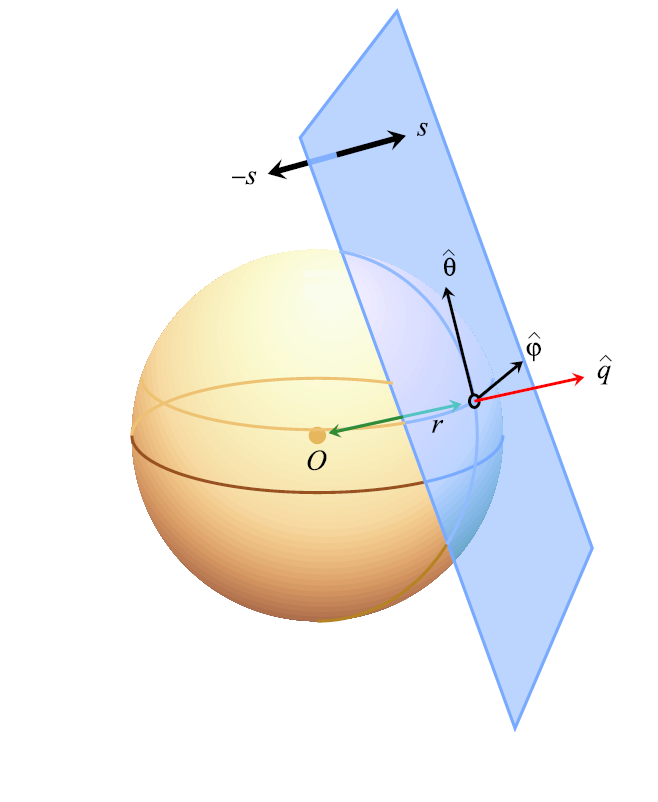
\includegraphics{images/img_15_2.png}
}
\caption{
\label{i15.2} Библейские (beables - хорошая идея, google-translate) значения для <<нейтрино>>, задаваемые как скаляр $r$ (расстояние плоскости от начала координат), булево $s$ и единичные векторы $\hat q$, $\hat \theta$ и $\hat \varphi$. $O$-это начало 3-мерного пространства}
\end {center}
\end {figure}

Обратите внимание, что вращение на $180^\circ$ вдоль оси, ортогональной к $\hat q$, может превратить $s$ в $-s$, что характерно для полунечетных спиновых представлений группы вращения, так что мы все еще можем рассматривать нейтрино как частицу спина $\frac 1 2$.\footnote{Но вращения в плоскости, или, что эквивалентно, вокруг оси $\hat q$, приводят к осложнениям, которые можно преодолеть, см. далее в этом разделе}

Здесь мы имеем представление о волновой функции для единственного «нейтрино» в необычном базисе. Как будет ясно из расчетов, представленных в подразделе ниже, в этом базисе «нейтрино» полностью не локализовано в двух поперечных направлениях, но его направление движения полностью фиксируется единичным вектором $\hat q$ и булевой переменной $s$. На этом основании «нейтрино» является детерминированным объектом. Вместо того, чтобы говорить, что у нас есть частица, мы говорим, что у нас есть плоский лист, плоскость. Единичный вектор $\hat q$ описывает ориентацию плоскости, а переменная $s$ сообщает нам, в каком из двух возможных направлений плоскость движется, всегда со скоростью света. Нейтрино - это детерминированные плоскости или плоские листы. Базис, в котором операторы $\hat q$, $r$ и $s$ диагональны, будет служить онтологическим базисом.

Наконец, мы могли бы использовать булеву переменную $s$ для определения знака $\hat q$, чтобы он стал более привычным единичным вектором, но это можно сделать лучше после того, как мы изучим операторы, которые переворачивают знак переменной $s$, с помощью небольшого усложнения, которое обсуждается, в разд. \ref{ch15.2.1} и \ref{ch15.2.2}.

Очевидно, что операторы, которые переворачивают знак $s$, существуют. Для этого возьмем любой вектор $\hat q'$, ортогональный к $\hat q$. Тогда оператор $\hat q'\cdot \vec\sigma$ подчиняется ($(\hat q'\cdot \vec\sigma) s = -s(\hat q'\cdot \vec\sigma)$, что легко проверить. Итак, этот оператор переворачивает знак. Проблема состоит в том, что в каждой точке сферы значений $\hat q$ можно взять суперпозицию любой такой единичной длины двух таких векторов $\hat q'$, ортогональных $\hat q$. Какой из них мы должны взять? Независимо от нашего выбора, это зависит от углов $\theta$ и $\phi$. Это подразумевает, что мы обязательно введем некоторую довольно неприятную угловую зависимость. Это оправдано тем, что исходное нейтрино имело спин $\frac 1 2$, и мы не можем имитировать это поведение с точки зрения зависимости $\hat q$, поскольку все волновые функции имеют интегральные вращение. Необходимо помнить об этом всякий раз, когда матрицы Паули обрабатываются в наших описаниях.

Таким образом, чтобы завершить нашу операторную алгебру в базисе, определяемом собственными значениями $\hat q$, $s$ и $r$, введем два новых оператора, квадраты которых равны одному. Определим два вектора, ортогональных к $\hat q$, один в направлении $\theta$ и один в направлении $\phi$:

\begin{equation}\label{15.29}
	\begin{array}{l}{\hat{q}=\left(\begin{array}{l}{q_{1}} \\ {q_{2}} \\ {q_{3}}\end{array}\right), \quad \quad \hat{\theta}=\frac{1}{\sqrt{q_{1}^{2}+q_{2}^{2}}}\left(\begin{array}{c}{q_{3} q_{1}} \\ {q_{3} q_{2}} \\ {q_{3}^{2}-1}\end{array}\right)} \\ {\hat{\varphi}=\frac{1}{\sqrt{q_{1}^{2}+q_{2}^{2}}}\left(\begin{array}{c}{-q_{2}} \\ {q_{1}} \\ {0}\end{array}\right)}\end{array}
\end{equation}

Все три нормированы на единицу, на что указывает каретка. Их компоненты подчиняются

\begin{equation}\label{15.30}
	q_{i}=\varepsilon_{i j k} \theta_{j} \varphi_{k}, \quad \theta_{i}=\varepsilon_{i j k} \varphi_{j} q_{k}, \quad \varphi_{i}=\varepsilon_{i j k} q_{j} \theta_{k}
\end{equation}

Затем мы определяем два оператора переключения знака: запишем $s = s_3$, затем

\begin{equation}\label{15.31}
	s_{1}=\hat{\theta} \cdot \vec{\sigma}, \quad s_{2}=\hat{\varphi} \cdot \vec{\sigma}, \quad s_{3}=s=\hat{q} \cdot \vec{\sigma}
\end{equation}

Они подчиняются

\begin{equation}\label{15.32}
	s_{i}^{2}=\mathbb{I}, \quad s_{1} s_{2}=i s_{3}, \quad s_{2} s_{3}=i s_{1}, \quad s_{3} s_{1}=i s_{2}
\end{equation}
                          
Рассматривая теперь beable операторы $\hat q$, $r$ и $s_3$, оператор преобразования $p_r$ для переменной $r$, операторы переворота спина (<<changeables>>) $s_1$ и $s_2$ и операторы вращения для единичного вектора $\hat q$, как мы можем преобразовать обратно в обычные нейтринные операторы $\vec x$, $\vec p$ и $\vec \sigma$?
Получить операторы импульса просто:

\begin{equation}\label{15.33}
	p_i = p_r \hat q_i
\end{equation}
            
а также матрицы Паули $\sigma_i$ могут быть выражены через $s_i$, просто обращая уравнения (\ref{15.31}). Используя уравнения (\ref{15.29}) и тот факт, что $q_1^2 + q_2^2 + q_3^2 = 1$, легко проверить, что

\begin{equation}\label{15.34}
	\sigma_{i}=\theta_{i} s_{1}+\varphi_{i} s_{2}+q_{i} s_{3}
\end{equation}
         
Тем не менее, получить операторы $x_i$ немного сложнее; они должны коммутировать с $\sigma_i$. Для этого нам сначала понадобятся операторы вращения $\vec L^{ont}$. Это не стандартный орбитальный или суммарный угловой момент. Наше преобразование из стандартных переменных в реальные переменные не будет достаточно инвариантным относительно вращения, просто потому, что мы будем использовать либо оператор $s_1$, либо оператор $s_2$ для перехода от нейтрино, движущегося влево, к движущемуся вправо. Обратите внимание, что на стандартной картине хиральные нейтрино имеют спин $\frac 1 2 $. Так что, при переходе от одного режима к противоположному требуется одна единица $\hbar$ углового момента в плоскости. Онтологический базис не относится к спину нейтрино, и именно поэтому наша алгебра дает некоторое ложное нарушение углового момента. Пока нейтрино не взаимодействуют, этот эффект остается практически незаметным, но необходимо проявлять осторожность, когда вводятся взаимодействия или масса.

Единственные операторы вращения, с которых мы можем поработать в рамках beable, это операторы, которые вращают плоскости относительно начала координат. Их мы называем $\vec L^{ont}$:

\begin{equation}\label{15.35}
	L_{i}^{\text {ont }}=-i \varepsilon_{i j k} q_{j} \frac{\partial}{\partial q_{k}}
\end{equation}

По определению, они коммутируют с $s_i$, но необходимо соблюдать осторожность на экваторе, где у нас есть граничное условие, которое лучше всего понять, наложив условие симметрии (\ref{15.18}).

Обратите внимание, что операторы $L_i^{ont}$ определенные в формуле (\ref{15.35}) не совпадают ни с одним из обычных операторов углового момента, потому что они не коммутируют с $s_i$, так как последние зависят от $\hat \theta$ и $\hat \varphi$. Найдем следующую связь между моментом импульса $\vec L$ нейтрино и $\vec L^{ont}$:

\begin{equation}\label{15.36}
	L_{i}^{\mathrm{ont}} \equiv L_{i}+\frac{1}{2}\left(\theta_{i} s_{1}+\varphi_{i} s_{2}-\frac{q_{3} \theta_{i}}{\sqrt{1-q_{3}^{2}}} s_{3}\right)
\end{equation}

вывод этого уравнения переносится в разд. \ref{ch15.21}.
Поскольку $\vec J = \vec L + \frac 1 2\vec\sigma$, можно также написать, используя уравнения (\ref{15.34}) и (\ref{15.29}),

\begin{equation}\label{15.37}
	L_{i}^{\mathrm{ont}}=J_{i}-\frac{1}{1-q_{3}^{2}}\left(\begin{array}{c}{q_{1}} \\ {q_{2}} \\ {0}\end{array}\right) s_{3}
\end{equation}

Затем мы выводим, в разделе \ref{ch15.2.1}, уравнение (\ref{15.60}), следующее выражение для операторов $x_i$ волновой функции нейтрино в терминах beables $\hat q$, $r$ и $s_3$ и changeables\footnote{См. (\ref{15.47}) и сделанные там замечания относительно определения оператора $1/p_r$ в мире библейских операторов, а также в конце раздела. \ref{ch15.2.2}.} $L_k^{ont}$, $p_r$, $s_1$ и $s_2$:

\begin{equation}\label{15.38}
	\begin{aligned} x_{i}=& q_{i}\left(r-\frac{i}{p_{r}}\right)+\varepsilon_{i j k} q_{j} L_{k}^{\text {ont }} / p_{r} \\ &+\frac{1}{2 p_{r}}\left(-\varphi_{i} s_{1}+\theta_{i} s_{2}+\frac{q_{3}}{\sqrt{1-q_{3}^{2}}} \varphi_{i} s_{3}\right) \end{aligned}
\end{equation}

(обратите внимание, что $\theta_i$ и $\phi_i$ являются beables, поскольку они являются функциями от $\hat q$).
Полное преобразование из библейского базиса (хорошо звучит) в один из общепринятых:

\begin{equation}\label{15.39}
	\left\langle\vec{p}, \alpha | \hat{q}, p_{r}, s\right\rangle= p_{r} \delta^{3}\left(\vec{p}-\hat{q} p_{r}\right) \chi_{\alpha}^{s}(\hat{q})
\end{equation}
            
где $\alpha$ - спиновый индекс волновых функций в базисе, где $\sigma_3$ - диагональ, а $\chi^s_\alpha$ - стандартное спинорное решение для уравнения $(\hat q \cdot \vec\sigma_{\alpha\beta})\chi^s_\beta(\hat q) = s\chi^s_\alpha(\hat q)$

В разделе \ref{ch15.2.2}, мы показываем, как это уравнение можно использовать для получения элементов матрицы унитарного преобразования, отображающей исходный базис в стандартную систему координат базиса волновых функций нейтрино\footnote{В этом выражении нет необходимости симметрировать $\hat q\cdot \vec x$, потому что и $\hat q$, и $\vec x$ состоят только из $C$-чисел.} (см. Уравнение \ref{15.83}):

\begin{equation}\label{15.40}
	\langle\vec{x}, \alpha | \hat{q}, r, s\rangle=\frac{i}{2 \pi} \delta^{\prime}(r-\hat{q} \cdot \vec{x}) \chi_{\alpha}^{s}(\hat{q})
\end{equation}

где $\delta\prime(z) \equiv \frac{d}{dz}\delta z$. Эта производная вылезает из множителя $p_r$ в формуле (\ref{15.39}), что необходимо для правильной нормализации состояния.

\subsubsection{Алгебра библейских «нейтринных» операторов}\label{ch15.2.1}

Этот подраздел довольно технический и может быть пропущен при первом чтении. Он выводит результаты, упомянутые в предыдущем разделе, обрабатывая алгебру, необходимую для преобразований из $(\hat q, s, r)$ базиса в ($\vec x$, $\sigma_3$) или ($\vec p$, $\sigma_3$) и обратно. Эта алгебра довольно сложна, опять же, потому что в beable представлении нет прямой ссылки на спин нейтрино. Хиральные нейтрино обычно снабжены спином $+\frac 1 2$ или $-\frac 1 2$ с осью вращения в направлении движения. Плоскости, которые движутся здесь, являются инвариантными относительно поворотов вокруг ортогональной оси, и связанный с ними вращательный момент не оставляет следа на невзаимодействующей, beable картине.

Это заставляет нас ввести некоторую ось внутри каждой плоскости, которая определяет фазы квантовых состояний, и эти (ненаблюдаемые) фазы явно нарушают инвариантность вращения.

Мы рассматриваем состояния, задаваемые переменными $s$ и $r$, а также полярные координаты $\theta$ и $\varphi$ для библовского $\hat q$ в областях, задаваемых уравнениями (\ref{15.23}), (\ref{15.24}). Таким образом, мы имеем состояния $|\theta,\varphi, s, r\rangle$. Как их можно выразить через более знакомые состояния $|\vec x,\sigma_z\rangle$ и / или $|\vec p,\sigma_z\rangle$, где $\sigma_z = \pm 1$ описывает спин нейтрино в направлении $z$ и наоборот?

Наши онтологические состояния задаются в онтологическом базисе, охватываемом операторами $\hat q$, $s (= s_3)$ и $r$. Мы добавим операторы (changeables) $s_1$ и $s_2$ (\ref{15.32}) и оператор

\begin{equation}\label{15.41}
	p_{r}=-i \partial / \partial r ; \quad\left[r, p_{r}\right]=i
\end{equation}

Исходные операторы импульса затем легко извлекаются. Как и в (\ref{15.17}), определим

\begin{equation}\label{15.42}
	\vec p = p_r \hat q
\end{equation}

Следующие операторы, которые мы можем воспроизвести из beable операторов $\hat q$, $r$ и $s_{1,2,3}$, это операторы Паули $\sigma_{1,2,3}$:

\begin{equation}\label{15.43}
	\sigma_{i}=\theta_{i} s_{1}+\varphi_{i} s_{2}+q_{i} s_{3}
\end{equation}

Обратите внимание, что теперь они нетривиально зависят от угловых параметров $\theta$ и $\varphi$, поскольку векторы $\hat\theta$ и $\hat\varphi$  определены в формуле (\ref{15.29}), нетривиально зависят от $\hat q$, который является радиальным вектором, задаваемым углами $\theta$ и $\varphi$. Легко проверить, что простые правила умножения из формул (\ref{15.32}) и правосторонняя ортонормированность (\ref{15.30}) гарантируют, что эти матрицы Паули также подчиняются правилам умножения. Учитывая тривиальные правила коммутации для beables, $[q_i, \theta_j] = [q_i, \varphi_j] = 0$ и $[p_r, q_i] = 0$, можно найти, что $[p_i, \sigma_j] = 0$, поэтому здесь у нас пока особых трудностей не возникает.
Все гораздо сложнее и деликатнее для операторов $x$. Чтобы восстановить оператор $\vec x = i\partial / \partial\vec p$, подчиняющийся $[x_i, p_j] = i\delta_{ij}$ и $[x_i, a_j] = 0$, сначала введем оператор орбитального углового момента

\begin{equation}\label{15.44}
	L_{i}=\varepsilon_{i j k} x_{i} p_{k}=-i \varepsilon_{i j k} q_{j} \frac{\partial}{\partial q_{k}}
\end{equation}

(где $\sigma_i$ сохраняются фиксированными), подчиняясь обычным правилам коммутации

\begin{equation}\label{15.45}
	\left[L_{i}, L_{j}\right]=i \varepsilon_{i j k} L_{k}, \quad\left[L_{i}, q_{j}\right]=i \varepsilon_{i j k} q_{k}, \quad\left[L_{i}, p_{j}\right]=i \varepsilon_{i j k} p_{k}, \text { etc. }
\end{equation}

в то время как $[L_i, \sigma_j] = 0$. Обратите внимание, что эти операторы не совпадают с угловым моментом $L_i^{ont}$ из (\ref{15.35}), поскольку те коммутируют с $s_j$, в то время как орбитальные угловые импульсы $L_i$; коммутируют с $\sigma_j$. В терминах орбитальных угловых моментов (\ref{15.44}) мы теперь можем восстановить исходные пространственные операторы $x_i$, $i = 1,2,3$, для нейтринос:

\begin{equation}\label{15.46}
	x_{i}=q_{i}\left(r-\frac{i}{p_{r}}\right)+\varepsilon_{i j k} q_{j} L_{k} / p_{r}
\end{equation}

Оператор $1 / p_r$, обратный оператору $ p_r = -i\partial / \partial r$, должен быть равным $-i$ множимой на оператор интегрирования. Это оставляет вопрос о постоянной интегрирования. Определить ее в импульсном пространстве несложно, но в конечном итоге $r$ является нашим beable оператором. Для волновых функций в $r$-пространстве $\psi(r,\ldots) = \langle r, \ldots |\psi\rangle$ где эллипсы стоят за другими beables (конечно, коммутируя с $r$), наиболее осторожное определение:

\begin{equation}\label{15.47}
	\frac{1}{p_{r}} \psi(r) \equiv \int_{-\infty}^{\infty} \frac{1}{2} i \operatorname{sgn}\left(r-r^{\prime}\right) \psi\left(r^{\prime}\right) \mathrm{d} r^{\prime}
\end{equation}

которое, как легко заметить, возвращает $\psi(r)$, когда $p_r$ действует на него. «$sgn(x)$» обозначает знак $х$. Отметим, что интеграл должен сходиться при $r\rightarrow \pm \infty$. Это ограничение на класс разрешенных волновых функций: в импульсном пространстве $\psi$ должно исчезать при $p_r\rightarrow 0$. Ограничения такого рода будут встречаться чаще в этой книге.

Антиэрмитский множитель $-i/p_r$ в формуле (\ref{15.46}) возникает автоматически при тщательном вычислении, и это просто компенсирует неэрмитичность последнего слагаемого, где $q_j$ и $L_k$ должны быть симметризованы, чтобы получить эрмитово выражение. $L_k$ коммутирует с $p_r$. В конце концов, $x_i$, определенный здесь, оказывается эрмитовым.

Возможно, это выглядело не слишком сложно, но это пока не все. Операторы $L_i$ коммутируют с $\sigma_j$, но не с beable переменными $s_i$. Таким образом, наблюдателю beable состояний в базисе beable будет трудно идентифицировать наши операторы $L_i$. Это будет легко для простого оператора, который задает операторы $L_i^{ont}$, которые генерируют вращения переменных $q_i$, коммутируя с $s_i$. Он мог бы также захотеть вращать Паули-подобные переменные $s_i$, используя оператор вращения, такой как $\frac 1 2 s_i$, но это не сработает, во-первых, потому что они больше не относятся, очевидно, к вращению, но, прежде всего, потому что $s_i$ в обычном базисе имеют гораздо меньшую тривиальную зависимость от углов $\theta$ и $\varphi$, см. уравнения (\ref{15.29}) и (\ref{15.31}).

На самом деле, восстановление операторов $\vec x$ из beables покажет нетривиальную зависимость от переменных $s_i$ и углов $\theta$ и $\varphi$. Это потому, что $\vec x$ и $s_i$ не коммутируют. Из определений (\ref{15.29}) и выражений для векторов $\hat\theta$ и $\hat\varphi$ вытекает:

\begin{equation}\label{15.48}
	\left[x_{i}, \theta_{j}\right]=\frac{i}{p_{r}}\left(\frac{q_{3}}{\sqrt{1-q_{3}^{2}}} \varphi_{i} \varphi_{j}-\theta_{i} q_{j}\right)
\end{equation}

\begin{equation}\label{15.49}
	\begin{aligned}
&\left[x_{i}, \varphi_{j}\right]=\frac{-i \varphi_{i}}{p_{r}}\left(q_{j}+\frac{\theta_{j} q_{3}}{\sqrt{1-q_{3}^{2}}}\right)\\
&\left[x_{i}, q_{j}\right]=\frac{i}{p_{r}}\left(\delta_{i j}-q_{i} q_{j}\right)
\end{aligned}
\end{equation}

Выражение $q_3/ \sqrt{1 - q^2_3} = \cot (\theta)$, возникающее здесь, является сингулярным на полюсах, очевидно, что из-за вихрей существуют определения угловых направлений $\theta$ и $\varphi$.

Из этих выражений мы теперь выводим коммутаторы $x_i$ и $s_{1, 2, 3}$:

\begin{equation}\label{15.51}
	\begin{aligned}
&\left[x_{i}, s_{1}\right]=\frac{i}{p_{r}}\left(\frac{\varphi_{i} q_{3}}{\sqrt{1-q_{3}^{2}}} s_{2}-\theta_{i} s_{3}\right)\\
&\left[x_{i}, s_{2}\right]=\frac{-i}{p_{r}} \varphi_{i}\left(s_{3}+\frac{q_{3}}{\sqrt{1-q_{3}^{2}}} s_{1}\right)\\
&\left[x_{i}, s_{3}\right]=\frac{i}{n}\left(\sigma_{i}-q_{i} s_{3}\right)=\frac{i}{n}\left(\theta_{i} s_{1}+\varphi_{i} s_{2}\right)
\end{aligned}
\end{equation}

В последнем выражении было использовано Eq. (\ref{15.43}) для $\vec\sigma$. Теперь заметим, что эти уравнения можно записать более компактно:

\begin{equation}\label{15.54}
	\left[x_{i}, s_{j}\right]=\frac{1}{2}\left[\frac{1}{p_{r}}\left(-\varphi_{i} s_{1}+\theta_{i} s_{2}+\frac{q_{3} \varphi_{i}}{\sqrt{1-q_{3}^{2}}} s_{3}\right), s_{j}\right]
\end{equation}

Чтобы действовать правильно, нам теперь нужно также знать, как операторы углового момента $L_i$ коммутируют с $s_{1, 2, 3}$. Запишем $L_i = \varepsilon_{ijk} x_j \hat q_k p_r$, где только функции $x_i$ не коммутируют с $s_j$. Тогда легко используя (\ref{15.51}) - (\ref{15.54}) находим нужные коммутаторы:

\begin{equation}\label{15.55}
	\left[L_{i}, s_{j}\right]=\frac{1}{2}\left[-\theta_{i} s_{1}-\varphi_{i} s_{2}+\frac{q_{3} \theta_{i}}{\sqrt{1-q_{3}^{2}}} s_{3}, s_{j}\right]
\end{equation}

где мы использовали простые соотношения ортонормированности (\ref{15.30}) для единичных векторов $\hat \theta$, $\hat \varphi$ и $\hat q$. Теперь это означает, что мы можем найти новые операторы $L_i^{ont}$, которые коммутируют со всеми $s_j$:

\begin{equation}\label{15.56}
	L_{i}^{\mathrm{ont}} \equiv L_{i}+\frac{1}{2}\left(\theta_{i} s_{1}+\varphi_{i} s_{2}-\frac{q_{3} \theta_{i}}{\sqrt{1-q_{3}^{2}}} s_{3}\right), \quad\left[L_{i}^{\mathrm{ont}}, s_{j}\right]=0
\end{equation}

как было предвосхищено в формуле (\ref{15.36}). В таком случае представляет интерес проверка коммутатора двух новых операторов «углового момента». Мы знаем одно: согласно тождеству Якоби, коммутатор двух операторов $L_i^{ont}$ также должен коммутировать со всеми $s_j$. Теперь выражение (\ref{15.56}), кажется, единственным, которое имеет ожидаемую форму и коммутирует со всеми $s$ операторами. Поэтому можно ожидать, что коммутатор двух операторов $L^{ont}$ снова должен привести к оператору $L^{ont}$, потому что другие выражения не могут коммутировать со всеми $s$. Явный расчет
коммутатора немного неуклюж. Например, не следует забывать, что $L_i$ также нетривиально коммутирует с  $\cot(\theta)$

\begin{equation}\label{15.57}
	\left[L_{i}, \frac{q_{3}}{\sqrt{1-q_{3}^{2}}}\right]=\frac{i \varphi_{i}}{1-q_{3}^{2}}
\end{equation}

Но тогда, действительно, можно найти

\begin{equation}\label{15.58}
	\left[L_{i}^{\text {ont }}, L_{j}^{\text {ont }}\right]=i \varepsilon_{i j k} L_{k}^{\text {ont }}
\end{equation}

На правила коммутации с $q_i$ и с $r$ и $p_r$ не влияли дополнительные условия:

\begin{equation}\label{15.59}
	\left[L_{i}^{\mathrm{ont}}, q_{j}\right]=i \varepsilon_{i j k} q_{k}, \quad\left[L_{i}^{\mathrm{ont}}, r\right]=\left[L_{i}^{\mathrm{ont}}, p_{r}\right]=0
\end{equation}

Это подтверждает, что теперь у нас действительно есть генератор для вращения beables $q_i$, в то время как он не влияет на другие beables $s_i$, $r$ and $p_r$.

Таким образом, чтобы найти правильное выражение для операторов $\vec x$ в терминах beable переменных, мы заменим $L_i$ в формуле (\ref{15.46}) на $L_i^{ont}$, приводя к

\begin{equation}\label{15.60}
	\begin{aligned}
x_{i}=& q_{i}\left(r-\frac{i}{p_{r}}\right)+\varepsilon_{i j k} q_{j} L_{k}^{\text {ont }} / p_{r} \\
&+\frac{1}{2 p_{r}}\left(-\varphi_{i} s_{1}+\theta_{i} s_{2}+\frac{q_{3}}{\sqrt{1-q_{3}^{2}}} \varphi_{i} s_{3}\right)
\end{aligned}
\end{equation}

Это замечательное выражение показывает, что в терминах beable переменных координаты $\vec x$ претерпевают конечные, зависящие от угла смещения, пропорциональные нашим операторам переворота знака $s_1$, $s_2$ и $s_3$. Эти смещения происходят в плоскости. Однако оператор $1 / p_r$ делает что-то еще. Из уравнения (\ref{15.47}) мы заключаем, что в переменной $r$

\begin{equation}\label{15.61}
	\left\langle r_{1}\left|\frac{1}{p_{r}}\right| r_{2}\right\rangle=\frac{1}{2} i \operatorname{sgn}\left(r_{1}-r_{2}\right)
\end{equation}

Возвращаясь теперь к замечанию, сделанному ранее в этой главе, можно использовать оператор знака $s_3$ (или некоторую комбинацию трех переменных $s$), чтобы различать противоположные знаки операторов $\hat q$. В этом случае углы $\theta$ и $\varphi$ занимают области, более обычные для сферы $S_2$: $0 <\theta <\pi$ и $0 <\varphi \le 2\pi$. В этом случае операторы $s_{1,2,3}$ ссылаются на знаки $q_3$, $r$ и $p_r$. Не так много можно было бы получить с помощью такой записи.

Гамильтониан в общепринятом базисе

\begin{equation}\label{15.62}
	H=\vec{\sigma} \cdot \vec{p}
\end{equation}

Он является линейным по импульсам $p_i$, но также зависит от некоммутирующих матриц Паули $\sigma_i$. Вот почему традиционный базис нельзя использовать напрямую, чтобы увидеть, что это детерминированная модель. Теперь, в нашем онтологическом базисе, получается

\begin{equation}\label{15.63}
	H = sp_r
\end{equation}

Таким образом, он умножает одну переменную импульса на коммутирующий оператор $s$. Уравнение Гамильтона гласит:

\begin{equation}\label{15.64}
	\frac{\partial r}{\partial t} = s
\end{equation}

в то время как все другие beables остаются постоянными. Так наша модель нейтрино стала детерминированной. На основе состояний $|\hat q, r,s\rangle$ наша модель четко описывает плоские листы на расстоянии $r$ от начала координат, ориентированные в направлении единичного вектора $\hat q$, движущегося со скоростью света в поперечном направлении, заданном знаком $s$.

Как только мы определили на основе двух собственных значений $s$, два других оператора $s_1$ и $s_2$,  (см. (\ref{15.32}))

\begin{equation}\label{15.65}
	s_{1}=\left(\begin{array}{cc}
{0} & {1} \\
{1} & {0}
\end{array}\right), \quad s_{2}=\left(\begin{array}{cc}
{0} & {-i} \\
{i} & {0}
\end{array}\right), \quad s_{3}=s=\left(\begin{array}{cc}
{1} & {0} \\
{0} & {-1}
\end{array}\right)
\end{equation}

в базисе состояний $|r\rangle$ оператор $p_r = -i\partial / \partial r$, а в базисе $|\hat q\rangle$ операторы $L_i^{ont}$

\begin{equation}\label{15.66}
	\begin{aligned}
\left[L_{i}^{\text {ont }}, L_{j}^{\text {ont }}\right] &=i \varepsilon_{i j k} L_{k}^{\text {ont }}, \quad\left[L_{i}^{\text {ont }}, q_{j}\right]=i \varepsilon_{i j k} q_{k} \\
\left[L_{i}^{\text {ont }}, r\right] &=0, \quad\left[L_{i}^{\text {ont }}, s_{j}\right]=0
\end{aligned}
\end{equation}
                          
мы можем записать в «онтологическом» базисе обычные «нейтринные» операторы $\vec \sigma$ (уравнение (\ref{15.43})), $\vec x$ (уравнение (\ref{15.60})) и $\vec p$ (уравнение (\ref{15.42})). По построению они будут соответствовать правильным коммутационным соотношениям.


\subsubsection{Ортонормальность и трансформации бейбл-состояний <<нейтрино>>}\label{ch15.2.2}

Соотношения, которые мы сейчас хотим определить, являются скалярными произведениями

\begin{equation}\label{15.67}
	\left\langle\vec{x}, \sigma_{z} | \theta, \varphi, s, r\right\rangle \quad
\left\langle\vec{p}, \sigma_{z} | \theta, \varphi, s, r\right\rangle
\end{equation}

Состояния $|\theta, \varphi, s, r\rangle$ впредь будут записываться как $|\hat q, s, r\rangle$. Использование импульсных переменных $\hat q \equiv \pm \vec p/|p|$, $q_z> 0$ вместе с вещественным параметром в скобке Дирака всегда будет означать beable состояние в этом подразделе.

Особое внимание требуется для правильной нормализации различных наборов собственных состояний. Мы предполагаем следующие нормализации:

\begin{equation}\label{15.68}
	\begin{aligned}
\left\langle\vec{x}, \alpha | \vec{x}^{\prime}, \beta\right\rangle &=\delta^{3}\left(\vec{x}-\vec{x}^{\prime}\right) \delta_{\alpha \beta} \\
\left\langle\vec{p}, \alpha | \vec{p}^{\prime}, \beta\right\rangle &=\delta^{3}\left(\vec{p}-\vec{p}^{\prime}\right) \delta_{\alpha \beta} \\
\langle\vec{x}, \alpha | \vec{p}, \beta\rangle &=(2 \pi)^{-3 / 2} e^{i \vec{p} \cdot \vec{x}} \delta_{\alpha \beta} \\
\left\langle\hat{q}, r, s | \hat{q}^{\prime}, r^{\prime}, s^{\prime}\right\rangle &=\delta^{2}\left(\hat{q}, \hat{q}^{\prime}\right) \delta\left(r-r^{\prime}\right) \delta_{s s^{\prime}} \\
\delta^{2}\left(\hat{q}, \hat{q}^{\prime}\right) & \equiv \frac{\delta\left(\theta-\theta^{\prime}\right) \delta\left(\varphi-\varphi^{\prime}\right)}{\sin \theta}
\end{aligned}
\end{equation}


$\alpha$ и $\beta$ - собственные значения матрицы Паули $\sigma_3$; далее,

\begin{equation}\label{15.73}
	\begin{aligned}
\int \delta^{3} \vec{x} \sum_{\alpha}|\vec{x}, \alpha\rangle\langle\vec{x}, \alpha| &=\mathbb{I}=\int \mathrm{d}^{2} \hat{q} \int_{-\infty}^{\infty} \mathrm{d} r \sum_{s=\pm}|\hat{q}, r, s\rangle\langle\hat{q}, r, s|; \\
\int \mathrm{d}^{2} \hat{q} & \equiv \int_{0}^{\pi / 2} \sin \theta \mathrm{d} \theta \int_{0}^{2 \pi} \mathrm{d} \varphi
\end{aligned}
\end{equation}

Различные матричные элементы теперь просты для вычисления. Сначала определим спиноры $\chi_\alpha^\pm(\hat q)$ решая

\begin{equation}\label{15.74}
	\left(\hat{q} \cdot \vec{\sigma}_{\alpha \beta}\right) \chi_{\beta}^{s}=s \chi_{\alpha}^{s} ; \quad\left(\begin{array}{cc}
{q_{3}-s} & {q_{1}-i q_{2}} \\
{q_{1}+i q_{2}} & {-q_{3}-s}
\end{array}\right)\left(\begin{array}{c}
{\chi_{1}^{s}} \\
{\chi_{2}^{s}}
\end{array}\right)=0
\end{equation}

что после нормализации спиноров 

\begin{equation}\label{15.75}
	\begin{aligned}
&\chi_{1}^{+}(\hat{q})=\sqrt{\frac{1}{2}\left(1+q_{3}\right)} ; \quad \chi_{1}^{-}(\hat{q})=-\sqrt{\frac{1}{2}\left(1-q_{3}\right)}\\
&\chi_{2}^{+}(\hat{q})=\frac{q_{1}+i q_{2}}{\sqrt{2\left(1+q_{3}\right)}} ; \quad \chi_{2}^{-}(\hat{q})=\frac{q_{1}+i q_{2}}{\sqrt{2\left(1-q_{3}\right)}}
\end{aligned}
\end{equation}

дает не только уравнение $s_3 \chi_\alpha^\pm = \pm \chi_\alpha^\pm$, но и

\begin{equation}\label{15.76}
	s_{1 \beta}^{\alpha} \chi_{\alpha}^{\pm}=\chi_{\beta}^{\mp}, \quad s_{2 \beta}^{\alpha} \chi_{\alpha}^{\pm}=\pm i \chi_{\beta}^{\mp}
\end{equation}
                           
что подразумевает ограничение на относительные фазы $\chi_\alpha^+$ и $\chi_\alpha^-$. Знак во втором из этих уравнений понимается, если мы разумеем, что индекс $s$ здесь, а позже в формуле. (\ref{15.80}), это верхний индекс.

Далее нам нужно знать, как нормализуются различные дельты Дирака:

\begin{equation}\label{15.77}
	\mathrm{d}^{3} \vec{p}=p_{r}^{2} \mathrm{d}^{2} \hat{q} \mathrm{d} p_{r} ; \quad \delta^{3}\left(\hat{q} p_{r}-\hat{q}^{\prime} p_{r}^{\prime}\right)=\frac{1}{p_{r}^{2}} \delta^{2}\left(\hat{q}, \hat{q}^{\prime}\right) \delta\left(p_{r}-p_{r}^{\prime}\right)
\end{equation}

Мы требуем, чтобы полнота означала

\begin{equation}\label{15.78}
	\begin{aligned}
&\int \mathrm{d}^{2} \hat{q} \int_{-\infty}^{\infty} \mathrm{d} p_{r} \sum_{s=\pm}\left\langle\vec{p}, \alpha | \hat{q}, p_{r}, s\right\rangle\left\langle\hat{q}, p_{r}, s | \vec{p}^{\prime}, \alpha^{\prime}\right\rangle=\delta_{\alpha \alpha^{\prime}} \delta^{3}\left(\vec{p}-\vec{p}^{\prime}\right)\\
&\int \mathrm{d}^{3} \vec{p} \sum_{\alpha=1}^{2}\left\langle\hat{q}, p_{r}, s | \vec{p}, \alpha\right\rangle\left\langle\vec{p}, \alpha | \hat{q}^{\prime}, p_{r}^{\prime}, s^{\prime}\right\rangle=\delta^{2}\left(\hat{q}, \hat{q}^{\prime}\right) \delta\left(p_{r}-p_{r}^{\prime}\right) \delta_{s s^{\prime}}
\end{aligned}
\end{equation}

как легко заметить \footnote{Обратите внимание, что фазы в этих элементах матрицы можно было определить по желанию, поэтому вместо $p_r$ мы выбрали $|p|$  для пущего удобства.}

\begin{equation}\label{15.80}
	\left\langle\vec{p}, \alpha | \hat{q}, p_{r}, s\right\rangle= p_{r} \delta^{3}\left(\vec{p}-\hat{q} p_{r}\right) \chi_{\alpha}^{s}(\hat{q})
\end{equation}
            
поскольку норма $p_r^2$ должна быть разделена на два матричных члена в уравнениях (\ref{15.78}) и (\ref{15.79}).

Это приводит нас к выводу, c использованием $\langle r \mid p_r \rangle = (2\pi)^{-1/2}e^{ip_r r}$,

\begin{equation}\label{15.81}
	\langle\vec{p}, \alpha | \hat{q}, r, s\rangle=\frac{1}{\sqrt{2 \pi}} \frac{1}{p_{r}} \delta^{2}\left(\frac{\pm \vec{p}}{|p|}, \hat{q}\right) e^{-i(\hat{q} \cdot \vec{p}) r} \chi_{\alpha}^{s}(\hat{q})
\end{equation}

      
где знак является знаком $р_3$.

Дельта Дирака здесь также может быть обозначена как

\begin{equation}\label{15.82}
	\delta^{2}\left(\frac{\pm \vec{p}}{|p|}, \hat{q}\right)=(\hat{q} \cdot \vec{p})^{2} \delta^{2}(\vec{p} \wedge \hat{q})
\end{equation}

где первый член является нормализацией, чтобы выражение стало масштабно-инвариантным, а второй просто заставляет $\vec p$ и $\hat q$ быть параллельными или антипараллельными. В случае $\hat q = (0,0, 1)$ оно просто описывает $p_3^2\delta(p_1)\delta(p_2)$.

Наконец, мы можем получить матричные элементы $\langle\vec x, \alpha\mid\hat q,r,s\rangle$. Просто временно, мы фиксируем $q$ в 3d-направлении: $\hat q = (0,0, 1)$,

\begin{equation}\label{15.83}
	\begin{aligned}
\langle\vec{x}, \alpha | \hat{q}, r, s\rangle &=\frac{1}{\sqrt{2 \pi}}(2 \pi)^{-3 / 2} \int \mathrm{d}^{3} \vec{p} \frac{(\hat{q} \cdot \vec{p})^{2}}{p_{r}} \delta^{2}(\vec{p} \wedge \hat{q}) e^{-i(\hat{q} \cdot \vec{p}) r+i \vec{p} \cdot \vec{x}} \chi_{\alpha}^{s}(\hat{q}) \\
&=\frac{1}{(2 \pi)^{2}} \int \mathrm{d}^{3} \vec{p} p_{3} \delta\left(p_{1}\right) \delta\left(p_{2}\right) e^{i p_{3}\left(x_{3}-r\right)} \chi_{\alpha}^{s}(\hat{q}) \\
&=\frac{1}{2 \pi} \frac{i \mathrm{d}}{\mathrm{d} r} \delta(r-\hat{q} \cdot \vec{x}) \chi_{\alpha}^{s}(\hat{q})=\frac{i}{2 \pi} \delta^{\prime}(r-\hat{q} \cdot \vec{x}) \chi_{\alpha}^{s}(\hat{q})
\end{aligned}
\end{equation}

С этими уравнениями наши законы преобразования теперь завершены. У нас есть все матричные элементы, чтобы показать, как перейти от одного базиса к другому. Отметим, что состояния с исчезающим $p_r$, импульсом листов, порождают сингулярности. Таким образом, мы видим, что состояния $|\psi\rangle$ с $\langle p_r = 0|\psi\rangle \neq 0$ или, что то же самое, $\langle \vec p = 0|\psi\rangle \neq 0$, должны быть исключены. Мы называем такие состояния <<граничными состояниями>>, поскольку они имеют волновые функции, которые постоянны в пространстве (в $r$, а также в $\vec x$), что означает, что они простираются до <<края>> вселенной. Здесь есть проблема, касающаяся граничных условий на бесконечности, которую нам нужно избегать. Мы видим, что оператор $1 / p_r$, уравнение (\ref{15.47}), плохо определен для этих состояний.









\subsubsection{Вторичное квантование «нейтрино»}\label{ch15.2.3}

Будучи релятивистским дираковским фермионом, объект, описанный в этой главе, страдает от проблемы, заключающейся в том, что его гамильтониан (\ref{15.25}) и (\ref{15.63}) не ограничен снизу. Существуют положительные и отрицательные энергетические состояния. Лечение будет таким же, как у Дирака, и мы будем использовать его позже: вторичное квантование. Мы следуем процедуре, описанной в разд. \ref{ch15.1}: для каждого данного значения единичного вектора $\hat q$ мы рассматриваем неограниченное количество «нейтрино», которые могут находиться в положительных или отрицательных энергетических состояниях. Чтобы быть более точным, можно временно поместить переменные $r$ в дискретную решетку:

\begin{equation}\label{15.84}
	r=r_{n}=n \delta r
\end{equation}


но часто мы игнорируем это, или другими словами, мы позволяем $\delta r$ стремиться к нулю.

Опишем эти частицы со спином $\frac 1 2$ антикоммутирующими фермионными операторами. У нас есть операторные поля $\psi_\alpha(\vec x)$ и $\psi^\dagger_\alpha(\vec x)$, подчиняющиеся правилам антикоммутации,                           

\begin{equation}\label{15.85}
	\left\{\psi_{\alpha}(\vec{x}), \psi_{\beta}^{\dagger}\left(\vec{x}^{\prime}\right)\right\}=\delta^{3}\left(\vec{x}-\vec{x}^{\prime}\right) \delta_{\alpha \beta}
\end{equation}
    
Используя правила преобразования из \ref{ch15.2.2}, мы можем преобразовать эти поля в поля $\psi(\hat{q}, r, s)$ и $\psi^{\dagger}\left(\hat{q}, r, s\right)$

\begin{equation}\label{15.86}
	\left\{\psi(\hat{q}, r, s), \psi^{\dagger}\left(\hat{q}^{\prime}, r^{\prime}, s^{\prime}\right)\right\}=\delta^{2}\left(\hat{q}, \hat{q}^{\prime}\right) \delta\left(r-r^{\prime}\right) \delta_{s s^{\prime}} \rightarrow \delta^{2}\left(\hat{q}, \hat{q}^{\prime}\right) \delta_{n n^{\prime}} \delta_{s s^{\prime}}
\end{equation}

При любом заданном значении $\hat q$ (которое также можно выбрать дискретным, если это необходимо), мы имеем прямую линию значений $r$, ограниченную точками решетки (\ref{15.84}). На отрезке $N$ узлов этой решетки мы можем представить любое количество фермионов в диапазоне от 0 до $N$. Каждый из этих фермионов подчиняется одному и тому же закону эволюции (\ref{15.64}), и поэтому также вся система является детерминированной.

Нет необходимости беспокоиться о введении антикоммутирующих фермионных операторов (\ref{15.85}), (\ref{15.86}). Знаки минус обрабатываются с помощью преобразования Jordan-Wigner, подразумевая, что создание или уничтожение фермиона, имеющего нечетное число предложений на одной стороне от него, будет сопровождаться искусственным знаком минус. Этот знак минус не имеет физического происхождения, но вводится исключительно для упрощения математики с антикоммутирующими полями. Поскольку при любом заданном значении $\hat q$ фермионы распространяются по одной линии и все они движутся с одинаковой скоростью в одном направлении, преобразование Джордана-Вигнера не вызывает затруднений. Конечно, мы еще не внедрили взаимодействия между фермионами, что на самом деле было бы непросто.

Эта <<вторично квантованная>> версия модели нейтрино имеет одно большое преимущество: мы можем описать ее с помощью гамильтониана, ограниченного снизу. Аргумент идентичен гениальной собственной процедуре Дирака. Гамильтониан вторично квантованной системы (сравните первый квантованный гамильтониан (\ref{15.25})):

\begin{equation}\label{15.87}
	H=\int \mathrm{d}^{3} \vec{x} \sum_{\alpha} \psi^{* \alpha}(\vec{x}) h_{\alpha}^{\beta} \psi_{\beta}(\vec{x}), \quad h_{\alpha}^{\beta}=-i \vec{\sigma}_{\alpha}^{\beta} \cdot \frac{\partial}{\partial \vec{x}}
\end{equation}
                        
Выполнение преобразования в beable базис, описанный в разд. \ref{ch15.2.2}, мы находим 

\begin{equation}\label{15.88}
	H=\int \mathrm{d}^{2} \hat{q} \int \mathrm{d} r \sum_{s} \psi^{*}(\hat{q}, r, s)(-i s) \frac{\partial}{\partial r} \psi(\hat{q}, r, s)
\end{equation}

Обозначим поле в стандартных обозначениях как $\psi^{stand}_\alpha(\vec x)$ или $\psi^{stand}_\alpha(\vec p)$, а поле в базисе 'beable' - $\psi^{\text{ont}}_s(\hat q, r)$. Его преобразование Фурье не является beable полем, но, чтобы отличить его от стандартных обозначений, мы иногда будем обозначать его как $\psi^{\text{ont}}_s(\hat q, p_r)$.
В импульсном пространстве мы имеем (см. Уравнение \ref{15.39}):

\begin{equation}\label{15.89}
	\begin{aligned}
\psi_{\alpha}^{\text {stand }}(\vec{p}) &=\frac{1}{p_{r}} \sum_{s} \chi_{\alpha}^{s}(\hat{q}) \psi_{s}^{\text {ont }}\left(\hat{q}, p_{r}\right) \\
\psi_{s}^{\text {ont }}\left(\hat{q}, p_{r}\right) &=p_{r} \sum_{\alpha} \chi_{\alpha}^{s}(\hat{q})^{*} \psi_{\alpha}^{\text {stand }}(\vec{p}), \quad \vec{p} \equiv \hat{q} p_{r}
\end{aligned}
\end{equation}
                          
где «stand» обозначает стандартное представление, а «ont» - онтологическое, хотя мы сделали преобразование Фурье, заменив переменную $r$ ее переменной импульса $p_r$. Нормализация такова, что

\begin{equation}\label{15.91}
	\sum_{\alpha} \int \mathrm{d}^{3} \vec{p}\left|\psi_{\alpha}^{\mathrm{stand}}(\vec{p})\right|^{2}=\sum_{s} \int_{\hat{q}_{3}>0} \mathrm{d}^{2} \hat{q} \int_{-\pi / \delta r}^{\pi / \delta r} \mathrm{d} p_{r}\left|\psi_{s}^{\mathrm{ont}}\left(\hat{q}, p_{r}\right)\right|^{2}
\end{equation}


см. уравнения (\ref{15.77}-\ref{15.80}).

В нашем случае $\psi$ имеет только два спиновых режима, это поле Вейля, но во всех других отношениях оно может обрабатываться так же, как безмассовое поле Дирака. Следуя Дираку, в импульсном пространстве каждый импульс $\vec p$ имеет две собственные моды энергии (собственные векторы оператора $j_\alpha^\beta$ в гамильтониане (\ref{15.87})), которые мы записали, должным образом нормированные как

\begin{equation}\label{15.92}
	u_{\alpha}^{\text {stand }\pm}(\vec{p})=\frac{1}{\sqrt{2|p|\left(|p| \pm p_{3}\right)}}\left(\begin{array}{c}
{\pm|p|+p_{3}} \\
{p_{1}+i p_{2}}
\end{array}\right) ; \quad E=\pm|p|
\end{equation}

Здесь спинор перечисляет значения для индекса $\alpha = 1,2$. В онтологическом базисе:

\begin{equation}\label{15.93}
	\begin{aligned}
u_{s}^{\text {ont } \pm}\left(\hat{q}, p_{r}\right) &=\left(\begin{array}{c}
{1} \\
{0}
\end{array}\right) & \text { if } \pm p_{r}>0, \quad\left(\begin{array}{l}
{0} \\
{1}
\end{array}\right) \quad \text { if } \pm p_{r}<0 \\
E &=\pm\left|p_{r}\right|
\end{aligned}
\end{equation}

            
Здесь спинор перечисляет значения для индекса $s = +$ и $-$.
В обоих случаях мы пишем



\begin{equation}\label{15.95}
	\begin{aligned}
\psi(\vec{p}) &=u^{+} a_{1}(\vec{p})+u^{-} a_{2}^{\dagger}(-\vec{p}) ; \quad\left\{a_{1}, a_{2}\right\}=\left\{a_{1}, a_{2}^{\dagger}\right\}=0 \\
\left\{a_{1}(\vec{p}), a_{1}^{\dagger}\left(\vec{p}^{\prime}\right)\right\} &=\left\{a_{2}(\vec{p}), a_{2}^{\dagger}\left(\vec{p}^{\prime}\right)\right\}=\delta^{3}\left(\vec{p}-\vec{p}^{\prime}\right) \text { or } \delta\left(p_{r}-p_{r}^{\prime}\right) \delta^{2}\left(\hat{q}, \hat{q}^{\prime}\right) \\
H^{\mathrm{op}} &=|p|\left(a_{1}^{\dagger} a_{1}+a_{2}^{\dagger} a_{2}-1\right)
\end{aligned}
\end{equation}

где $a_1$ - оператор аннигиляции для частицы с импульсом $\vec p$, а $a_2^\dagger$ - оператор рождения античастицы с импульсом $-\vec p$. Мы опускаем вакуумную энергию $-1$. В случае, если у нас есть решетка в $r$-пространстве, импульс ограничен значениями $|\vec p| = |p_r| < \pi/\delta_r$.


\subsection{Нейтринные вакуумные корреляции}\label{ch15.3}

Вакуумное состояние $|\emptyset\rangle$ является состоянием самой низкой энергии. Это означает, что при каждом значении импульса $\vec p$ или, что эквивалентно, при каждом $(\hat q, p_r)$ мы имеем

\begin{equation}\label{15.98}
	a_{i}|\emptyset\rangle= 0
\end{equation}

           
где $a_i$ - оператор аннигиляции для всех состояний с $H = \sigma\cdot\vec p = sp_r > 0$ и оператор создания, если $H <0$. Возможные состояния - это состояния, в которых при каждом значении набора $(\hat q, r, s)$ число «частиц» задается равным 1 или 0. Это, конечно, означает, что вакуумное состояние (\ref{15.98}) не beable; это суперпозиция всех возможных состояний.

Например, можно вычислить корреляционные функции движущихся справа и слева «частиц» (фактически, листов) в заданном направлении. В онтологическом базисе можно обнаружить, что левые двигатели не соотносятся с правыми, но два левых двигаются следующим образом:

\begin{equation}\label{15.99}
	\begin{array}{l}
{P\left(r_{1}, r_{2}\right)-P\left(r_{1}\right) P\left(r_{2}\right)} \\
{\quad=\delta r^{2}\left\langle\emptyset\left|\psi_{s}^{*}\left(r_{1}\right) \psi_{s}\left(r_{1}\right) \psi_{s}^{*}\left(r_{2}\right) \psi_{s}\left(r_{2}\right)\right| \emptyset\right\rangle_{\mathrm{conn}}} \\
{\quad=\left|\frac{\delta r}{2 \pi} \int_{0}^{\pi / \delta r} \mathrm{d} p e^{i p\left(r_{2}-r_{1}\right)}\right|^{2}=\left\{\begin{array}{cc}
{\frac{\delta r^{2}}{\pi^{2}\left|r_{1}-r_{2}\right|^{2}}} & {\text { if } \frac{r_{1}-r_{2}}{\delta r}=\operatorname{odd}} \\
{\frac{1}{4} \delta_{r_{1}, r_{2}}} & {\text { if } \frac{r_{1}-r_{2}}{\delta r}=\text { even }}
\end{array}\right.}
\end{array}
\end{equation}
 
где $\delta r^2$, единица расстояния между двумя соседними квадратами листов, была добавлена для нормализации, а «conn» обозначает только вклад в подключенную диаграмму, то есть частица и античастица, созданные в $r_2$, аннигилированы в $r_1$. Время применяется к двум правым движителям. В случае решетки, где $\delta r$ еще не настроен на ноль, этот расчет все еще точен, если $r_1 - r_2$ является целым кратным $\delta r$. Отметим, что для вакуума $P (r) = P (r, r) = \frac 1 2$.
Важный момент, касающийся второго квантованного гамильтониана (\ref{15.87}), (\ref{15.88}): на решетке мы хотим использовать гамильтониан (\ref{15.97}) в импульсном пространстве. В позиционном пространстве, уравнения (\ref{15.87}) или (\ref{15.88}) не могут быть действительными, поскольку нельзя дифференцировать в пространственной переменной $r$. Но мы можем иметь оператор индуктивности для конечных целочисленных интервалов времени $T = n_t\delta r$. Затем этот эволюционный оператор смещает левые двигатели на один шаг влево, а правые двигатели на один шаг вправо. Гамильтониан (\ref{15.84}) делает именно это, в то время как его можно использовать также для бесконечно малых времен; однако оно не совсем локально при повторном выражении в терминах полей на координатах решетки, поскольку теперь импульс ограничен пребыванием в зоне Бриллюэна $| p_r | <\pi / \delta р$. Эта особенность, которая здесь не приводит к серьезным осложнениям, дополнительно объясняется для бозонного случая в разд. \ref{ch17.1.1}

Корреляции данных в двух точках, которые разделены в пространстве, но не во времени, или недостаточно далеко в направлении времени, чтобы позволить световым сигналам соединять эти две точки, называются пространственно-подобными корреляциями. Пространственные корреляции, найденные в формуле. (\ref{15.99}) важны. Они, вероятно, играют важную роль в таинственном поведении beable моделей, когда рассматриваются неравенства Белла, см. Часть I, гл. \ref{ch17.1.1} и выше.

Обратите внимание, что здесь мы имеем дело с пространственно-подобными корреляциями онтологических степеней свободы. Корреляции являются следствием того факта, что мы смотрим на особое состояние, которое сохраняется во времени, состояние, которое мы называем вакуумом. Все физические состояния, которые обычно встречаются, являются шаблонными состояниями, лишь незначительно отклоняющимися от этого вакуумного состояния, поэтому у нас всегда будут такие корреляции.

В главах о неравенствах Белла и интерпретации клеточного автомата (раздел \ref{ch5.2} и глава \ref{ch3} части I) утверждается, что онтологические теории, предложенные в этой книге, должны иметь сильные пространственно-подобные корреляции во всей вселенной. Это был бы единственный способ объяснить, как неравенства Белла, или CHSH могут быть так сильно нарушены в этих моделях. Теперь, когда наши «нейтрино» не взаимодействуют, на самом деле нельзя проводить с ними ЭПР-подобные эксперименты, поэтому уже по этой причине прямого противоречия нет. Однако мы также видим, что в этой модели присутствуют сильные пространственно-подобные корреляции.
Действительно, первое впечатление может показаться, что онтологическая модель «нейтринного листа» предыдущего раздела полностью нелокальна. Листы простираются бесконечно далеко в двух направлениях, и если лист движется здесь, мы немедленно получаем некоторую информацию о том, что он делает в другом месте. Но при ближайшем рассмотрении следует признать, что уравнения движения полностью локальны. Эти уравнения говорят нам, что если у нас есть лист, проходящий через точку $x$ пространства-времени, несущий функцию знака $s$ и ориентированный в направлении $\hat q$, то в точке $x$ лист будет двигаться со скоростью света в продиктованном направлении по $\hat q$ и $\sigma$. Никакая информация не требуется от точек в другом месте во вселенной. Это локальность.

То, что не является локальным, - это повсеместные корреляции в этой модели. Если у нас есть лист в точке $(\vec x, t)$, ориентированный в направлении $\hat q$, мы сразу узнаем, что этот же лист будет находиться в других точках $(\vec y, t)$, если $\hat q \cdot (\vec y - \vec x) = 0$, и он имеет такие же значения для $\hat q$ и $\sigma$. В гл. \ref{ch20.7} выяснится, что пространственно-подобные корреляции являются нормальными в физике, как в классических системах, таких как кристаллы или звездные скопления, так и в квантово-механических, таких как квантованные поля. В нейтринных листах корреляции еще более сильны, так как их отсутствие является большой ошибкой, когда мы делаем выводы из теоремы Белла.

\end{document}

